\providecommand{\atd}{..}
\documentclass[../ATD.tex]{subfiles}

\begin{document}
    \chapter{Testing}\label{ch:testing}
    The application has some important issues and bugs.
    Only few functionality works properly, making it impossible to test all the features of the application.
    The requirements that we were not able to test are described in a dedicated section, with the reason of their failure.

    \section{Testing Requirements Table}\label{sec:testing-requirements-table}
    As already described, it will not be possible to test all the requirements since some of them will not be showed at all.
    Moreover, it will be difficult to follow the requirement order presented in the RASD and in the ITD, so the following table purpose is to show which requirements will be tested.
    At the end of the chapter a section for the untested requirements will be provided anyway.

    \begin{enumerate}
        \requirement{1} The reports about the violations are correctly stored.
        \requirement{2} The user can view the statistics calculated by the system with some exceptions.
        \requirement{3} The municipality can access only the data of the violations of its competence area.
        \requirement{4} Violations registered by the municipality can be retrieved by the system.
        \requirement{5} The system must avoid the manipulation of the violations.
        \requirement{6} The system must be able to retrieve the position from the user or from the GPS.
        \requirement{7} Only the municipality can access the submitted parking violation of its competence area.
        \requirement{8} The system must allow the user to take a picture or to select one from the device.
        \requirement{9} The system accepts reports from the user.
        \requirement{10} The system must calculate some statistics.
        \requirement{11} The municipality can view all the statistics calculated by the system.
        \requirement{12} The system must suggest interventions to the municipality.
        \requirement{13} The system accepts only reports with a valid plate number and position.
        \requirement{14} The system must allow the user to perform the registration and the login.
        \requirement{15} The system must allow the municipality to perform the registration and the login.
        \requirement{16} The system must ask the user the non-mandatory attributes of the report.
        \requirement{17} The system must communicate with the Identity Verifier.
        \requirement{18} The system must communicate with the Plate Recognizer Service.
        \requirement{19} The system must communicate with the Maps Service.
    \end{enumerate}
   %%todo ******** TABELLA *********
    %%traceability matrix
    \begin{adjustwidth}{+2cm}{}
        \begin{longtable}[H]
        {|| p{.10\linewidth} || p{.40\linewidth} ||
        p{.19\linewidth} | p{.13\linewidth} |}
            \hline
            \textbf{\makecell{R}} & \textbf{\makecell{Implemented}} & \textbf{\makecell{Tested}} \\ \hline
            \textbf{1}  & \textit{Yes}       & No  \\ \hline
            \textbf{2}  & \textit{Yes}       & Yes \\ \hline
            \textbf{3}  & \textit{Yes}       & Yes \\ \hline
            \textbf{4}  & \textit{No}        &  -  \\ \hline
            \textbf{5}  & \textit{Yes}       & No  \\ \hline
            \textbf{6}  & \textit{Yes}       & No  \\ \hline
            \textbf{7}  & \textit{Yes}       & Yes \\ \hline
            \textbf{8}  & \textit{Yes}       & Yes \\ \hline
            \textbf{9}  & \textit{Yes}       & Yes \\ \hline
            \textbf{10} & \textit{Yes}       & No  \\ \hline
            \textbf{11} & \textit{Yes}       & Yes \\ \hline
            \textbf{12} & \textit{No}        &  -  \\ \hline
            \textbf{13} & \textit{Partially} &  -  \\ \hline
            \textbf{14} & \textit{Yes}       & Yes \\ \hline
            \textbf{15} & \textit{Yes}       & Yes \\ \hline
            \textbf{16} & \textit{Yes}       & No  \\ \hline
            \textbf{17} & \textit{No}        &  -  \\ \hline
            \textbf{18} & \textit{No}        &  -  \\ \hline
            \textbf{19} & \textit{Yes}       & No  \\ \hline
            \caption[\textit{Traceability matrix}]{\textit{Traceability matrix}}
        \end{longtable}
    \end{adjustwidth}

    \section{Test Cases}\label{sec:test-cases}
    The test cases will be presented as follow: they will be group by tested requirements, and for every test will be described the following information:
    \begin{enumerate}
        \item \textbf{Test purpose}
        \item \textbf{Device}: device on which the test run (android phone, iOS phone, simulator, web page, etc..)
        \item \textbf{Input}: input of the test
        \item \textbf{Outcome}: output of the test
        \item \textbf{Result}: passed or fail
        \item (Eventually) \textbf{Possible bugs}: list of possible bugs
        \item (Eventually) \textbf{Comment}: relevant comments about the test
    \end{enumerate}
    As previously explained, it will not be possible to test the requirements in the same order as they are presented in the RASD and ITD,
    but they will be marked with the same enumeration to make them easier to read.
    The requirements will be marked \textbf{[Rn]}, to refer to the n-th requirement.

    \subsection{User registration and login R[14]}\label{subsec:user-registration-and-login}
    R14: The system must allow the user to perform the registration and the login.

    \subsubsection{User login 1}\label{subsubsec:user-login-1}
    \begin{itemize}
        \item \textbf{Test purpose}: An user that is already signed in must be able to login correctly.
        \item \textbf{Device}: iPhone
        \item \textbf{Input}: username: "jak4", password: "jak".
        \item \textbf{Outcome}: SafeStreet user's main menu.
        \item \textbf{Result}: Passed
        \item \textbf{Comment}: The user "jak4" was already registered with the password "jak".
    \end{itemize}

    \subsubsection{User login 2}\label{subsubsec:user-login-2}
    \begin{itemize}
        \item \textbf{Test purpose}: An user that is already signed in must be able to login correctly.
        \item \textbf{Device}: Web page (MacOS)
        \item \textbf{Input}: username: "jak4", password: "jak".
        \item \textbf{Outcome}: SafeStreet user's main menu.
        \item \textbf{Result}: Passed
        \item \textbf{Comment}: The user "jak4" was already registered with the password "jak".
    \end{itemize}

    \subsubsection{User login 3}\label{subsubsec:user-login-3}
    \begin{itemize}
        \item \textbf{Test purpose}: An user that is already signed in must be able to login correctly if the server is up.
        \item \textbf{Device}: iOS simulator
        \item \textbf{Input}: Server turned off, username: "jak4", password: "jak".
        \item \textbf{Outcome}: Nothing happen.
        \item \textbf{Result}: Passed
        \item \textbf{Comment}: Since the server is down, it is fine that nothing happen if i try to login.
    \end{itemize}

    \subsubsection{User login 4}\label{subsubsec:user-login-4}
    \begin{itemize}
        \item \textbf{Test purpose}: An user can not login with an unregistered account.
        \item \textbf{Device}: iOS simulator
        \item \textbf{Input}: username: "fakeTestAccount", password: "psw".
        \item \textbf{Outcome}: Invalid data message.
        \item \textbf{Result}: Passed
    \end{itemize}

    \subsubsection{User registration 1}\label{subsubsec:user-registration-1}
    \begin{itemize}
        \item \textbf{Test purpose}: An user must be allowed to register.
        The user try to register by providing all the information required.
        \item \textbf{Device}: iOS simulator
        \item \textbf{Input}: username: "test1", email: "test@test.it", name: "TestName", surname: "TestSurname", place of birth: "TestPlace", date of birth: "01-01-1001", place of residence: "TestPlace", fiscal code: "aaaaaaaaaaaaaaaa", password "testpsw", id photo: a picture from device, your photo: a picture from device
        \item \textbf{Outcome}: Nothing happen
        \item \textbf{Result}: Failed
        \item \textbf{Possible bugs}: The application does not perform any action, but on the intelliJ console it is possible to see an error "Unhandled Exception: FormatException: Invalid date format".
        \item \textbf{Comment}: Talking with the developer group, we know that the correct format for the date is yyyy-mm-dd.
        The application should inform the user about that restriction.
        Moreover, the application should show an error to inform the user that something went wrong, because it is not intuitive to understand that the sign up request has been sent.
    \end{itemize}

    \subsubsection{User registration 2}\label{subsubsec:user-registration-2}
    \begin{itemize}
        \item \textbf{Test purpose}: An user must be allowed to register.
        The user try to register by not giving any information.
        \item \textbf{Device}: iOS simulator
        \item \textbf{Input}: none
        \item \textbf{Outcome}: All the textual textfield are signed as mandatory.
        \item \textbf{Result}: Passed
        \item \textbf{Comment}: The "ID PHOTO" and "YOUR PHOTO" button are not marked as mandatory.
    \end{itemize}

    \subsubsection{User registration 3}\label{subsubsec:user-registration-3}
    \begin{itemize}
        \item \textbf{Test purpose}: An user must be allowed to register.
        The user try to register by giving all the information, except for the two pictures.
        \item \textbf{Device}: iOS simulator
        \item \textbf{Input}: username: "test1", email: "test@test.it", name: "TestName", surname: "TestSurname", place of birth: "TestPlace", date of birth: "1001-01-01", place of residence: "TestPlace", fiscal code: "aaaaaaaaaaaaaaaa", password "testpsw"
        \item \textbf{Outcome}: Nothing happen
        \item \textbf{Result}: Failed
        \item \textbf{Comment}: Nothing happen, but from the intelliJ console it is possible to see that the pictures are mandatory for the registration.
        They should be marked as mandatory as well as all the other fields, since it is not intuitive to understand what is going wrong.
    \end{itemize}

    \subsubsection{User registration 4}\label{subsubsec:user-registration-4}
    \begin{itemize}
        \item \textbf{Test purpose}: An user must be allowed to register.
        The user try to register by giving all the correct information.
        \item \textbf{Device}: iOS simulator
        \item \textbf{Input}: username: "test1", email: "test@test.it", name: "TestName", surname: "TestSurname", place of birth: "TestPlace", date of birth: "1001-01-01", place of residence: "TestPlace", fiscal code: "aaaaaaaaaaaaaaaa", password "testpsw", id photo: a picture from device, your photo: a picture from device
        \item \textbf{Outcome}: All the textual textfield are signed as mandatory.
        \item \textbf{Result}: Passed
        \item \textbf{Comment}: The "ID PHOTO" and "YOUR PHOTO" button are not marked as mandatory.
    \end{itemize}

    \subsubsection{User registration 5}\label{subsubsec:user-registration-5}
    \begin{itemize}
        \item \textbf{Test purpose}: An user must be allowed to register.
        The user try to register by giving all the correct information.
        \item \textbf{Device}: Web page (MacOS)
        \item \textbf{Input}: username: "test1", email: "test@test.it", name: "TestName", surname: "TestSurname", place of birth: "TestPlace", date of birth: "1001-01-01", place of residence: "TestPlace", fiscal code: "aaaaaaaaaaaaaaaa", password "testpsw"
        \item \textbf{Outcome}: The web page do not open neither the camera or the gallery.
        \item \textbf{Result}: Failed
        \item \textbf{Comment}: Since neither the camera or the gallery can be used to upload a picture, the registration can not be performed by the web page (the pictures are mandatory information for the registration).
    \end{itemize}

    \subsubsection{User registration 6}\label{subsubsec:user-registration-6}
    \begin{itemize}
        \item \textbf{Test purpose}: An user must be allowed to register.
        The user try to register by giving all the correct information.
        \item \textbf{Device}: iPhone
        \item \textbf{Input}: username: "federico111", email: "federico.innocente.spam@gmail.com", name: "Federico", surname: "Innocente", place of birth: "Pordenone", date of birth: "1997-06-19", place of residence: "Pordenone", fiscal code: "NNCFRC97H19G888Q", password "passwordP1", id picture: picture from camera, your picture: picture from camera.
        \item \textbf{Outcome}: Nothing happen
        \item \textbf{Result}: Failed
        \item \textbf{Comment}: I can assume that the registration failed, since I provided all real information and if I try to go back in sign in page and log in, a message said that I am using invalid email and password.
    \end{itemize}

    \subsection{Municipality registration and login [R15]}\label{subsec:municipality-registration-and-login}
    R15: The system must allow the Municipality to perform the registration and the login.

    \subsubsection{Municipality login 1}\label{subsubsec:municipality-login-1}
    \begin{itemize}
        \item \textbf{Test purpose}: A municipality that is already signed in must be able to login correctly.
        \item \textbf{Device}: iOS simulator
        \item \textbf{Input}: username: "Milano", password: "Milan".
        \item \textbf{Outcome}: SafeStreet municipality's main menu.
        \item \textbf{Result}: Passed
        \item \textbf{Comment}: The municipality "Milano" was already registered with the password "Milan".
    \end{itemize}

    \subsubsection{Municipality login 2}\label{subsubsec:municipality-login-2}
    \begin{itemize}
        \item \textbf{Test purpose}: An user that is already signed in must be able to login correctly.
        \item \textbf{Device}: Web page (MacOS)
        \item \textbf{Input}: username: "Milano", password: "Milan".
        \item \textbf{Outcome}: SafeStreet municipality's main menu.
        \item \textbf{Result}: Passed
        \item \textbf{Comment}: The user "Milano" was already registered with the password "Milan".
    \end{itemize}

    \subsubsection{Municipality registration}\label{subsubsec:municipality-registration}
    \begin{itemize}
        \item \textbf{Test purpose}: A municipality must be able to register itself on SafeStreets.
        \item \textbf{Device}: Web page (MacOS)
        \item \textbf{Input}: activation code: "123123123", username: "Test", password: "TestPsw".
        \item \textbf{Outcome}: Nothing happen.
        \item \textbf{Result}: Failed
    \end{itemize}

    \subsection{User statistics [R2]}\label{subsec:user-statistics}
    R2: The user can view the statistics calculated by the System with some exceptions.
    \newline
    R2.A: The vehicles that have committed the highest number of violations.
    \newline
    For the purpose of these tests, it is important to say that some violation was already stored in the database provided by the developer group.
    They are 19 violations, 17 reported for "PARKING\_ON\_RESERVED\_STALL" and 2 for "PARKING\_ON\_SIDEWALK", all uploaded between 12-10-2019 and 04-01-2020, according with the stored information.
    A picture of a query on the database is provided for more information:

    \begin{figure}[H]
        \centering
        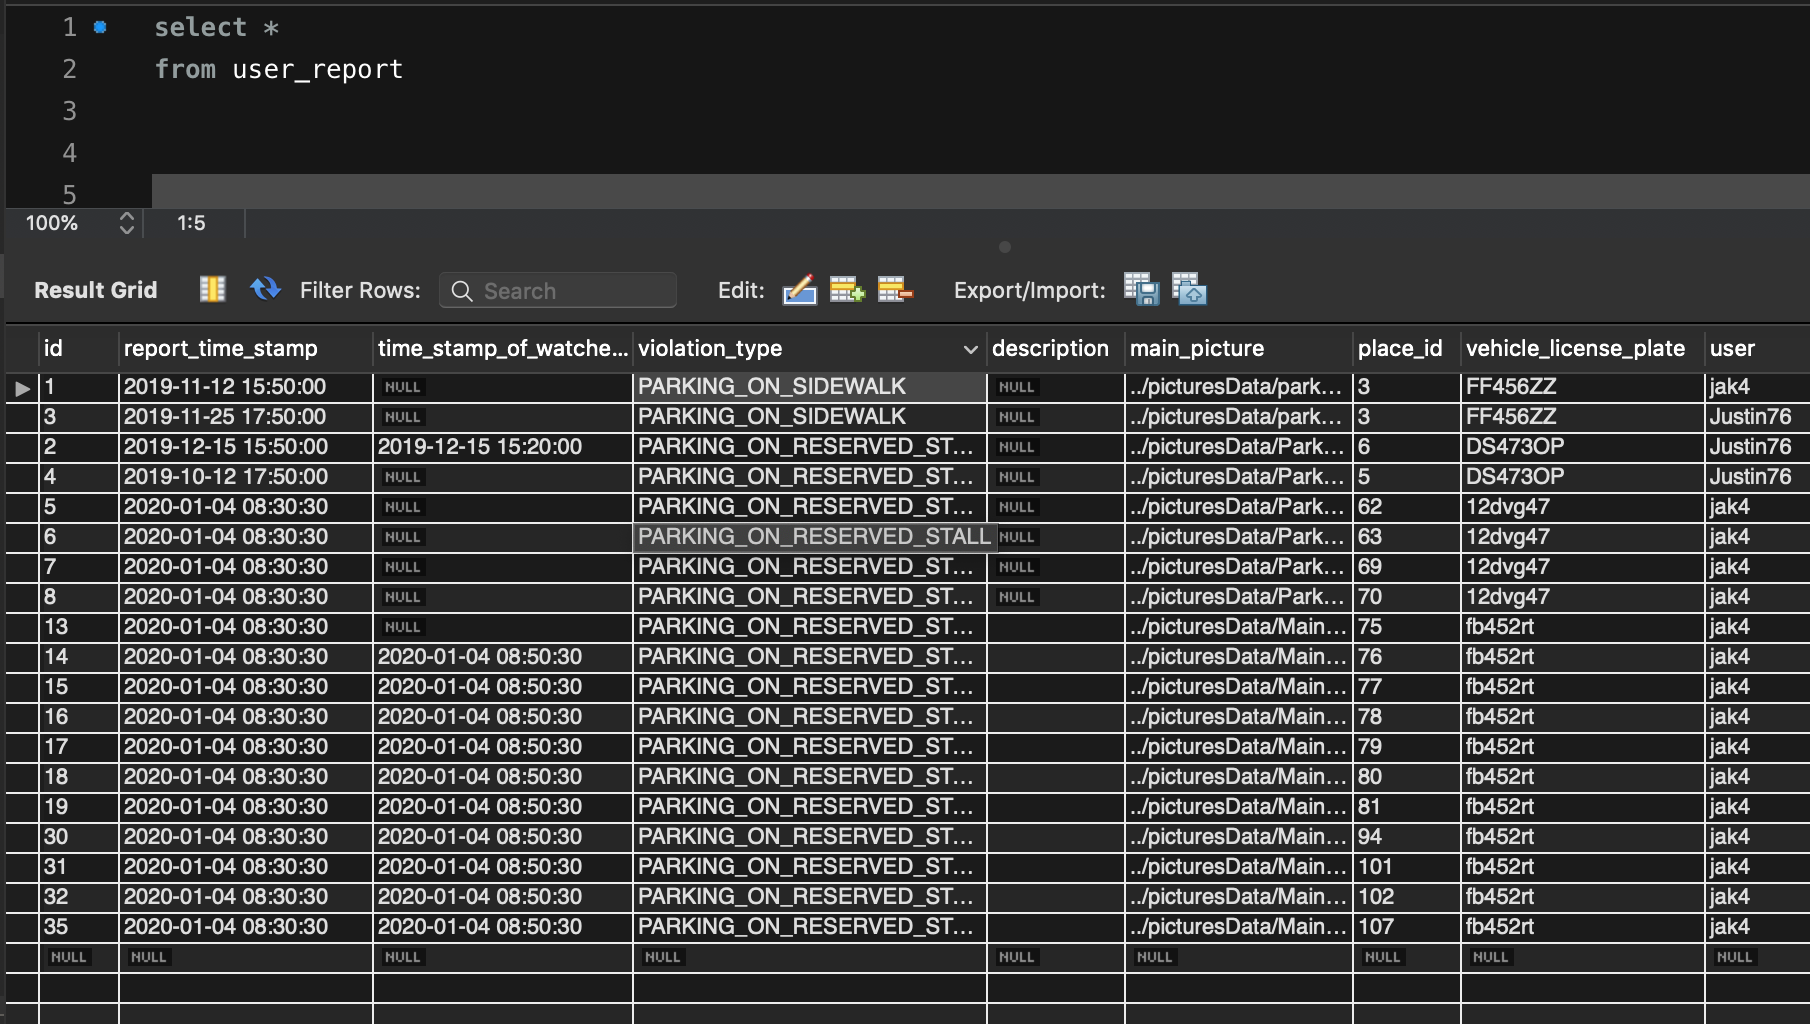
\includegraphics[scale = 0.5]{assets/database_user_report.png}\\
        \caption[Query on all the report stored]{Query on all the report stored.}
    \end{figure}

    \subsubsection{Statistics interrogation 1}\label{subsubsec:statistics-interrogation-1}
    \begin{itemize}
        \item \textbf{Test purpose}: An user must be able to view the statistics.
        \item \textbf{Device}: iPhone
        \item \textbf{Input}: "Effectiveness" choice in the drop down menu of the "Statistics" page.
        \item \textbf{Outcome}: Nothing happen.
        \item \textbf{Result}: Failed
        \item \textbf{Comment}: The same results can be obtained by choosing the "Streets with most violation" or "Most common violation" option.
    \end{itemize}

    \subsubsection{Statistics interrogation 2}\label{subsec:statistics-interrogation-2}
    \begin{itemize}
        \item \textbf{Test purpose}: An user must be able to view the statistics.
        \item \textbf{Device}: Web page (MacOS)
        \item \textbf{Input}: "Effectiveness" choice in the drop down menu of the "Statistics" page.
        \item \textbf{Outcome}: A button with a text description "Send default" appear, but than clicking on any point of the page (both the button or not), it disappear and nothing happen.
        \item \textbf{Result}: Failed
        \item \textbf{Comment}: The same results can be obtained by choosing the "Streets with most violation" or "Most common violation" option.
    \end{itemize}

    \subsection{Municipality violations access [R3]}\label{subsec:municipality-report-access}
    R3: The Municipality can access only the data of the violations of its competence area.
    \newline
    For the purpose of these tests, it is important to say that some violation was already stored in the database provided by the developer group.
    \subsubsection{Municipality violation request 1}\label{subsubsec:municiplaity-violation-request-1}
    \begin{itemize}
        \item \textbf{Test purpose}: The municipality can see all the violation reported on its territory.
        \item \textbf{Device}: iPhone
        \item \textbf{Input}: Milan municipality (username: "Milano", password: "Milan"), look for the violations from "01-11-2019" until "21-01-2020".
        \item \textbf{Outcome}: 17 violations are reported, all of them with the city marked as "Milano".
        \item \textbf{Result}: Passed
        \item \textbf{Bugs}: The first 7 violations are always marked as uploaded in the moment in which the query has been done (same day and hour).
        \item \textbf{Comment}: The date and time error is for sure a bug of the application, but it do not prevent the requirement from being satisfied.
    \end{itemize}

    \subsubsection{Municipality violation request 2}\label{subsubsec:municiplaity-violation-request-2}
    \begin{itemize}
        \item \textbf{Test purpose}: The municipality can see all the violation reported on its territory.
        \item \textbf{Device}: Web page (MacOS)
        \item \textbf{Input}: Milan municipality (username: "Milano", password: "Milan"), look for the violations from "01-110-2019" until "21-01-2020".
        \item \textbf{Outcome}: 17 violations are reported, all of them with the city marked as "Milano".
        \item \textbf{Result}: Passed
        \item \textbf{Bugs}: The first 7 violations are always marked as uploaded in the moment in which the query has been done (same day and hour).
        \item \textbf{Comment}: The date and time error is for sure a bug of the application, but it do not prevent the requirement from being satisfied.
    \end{itemize}

    \subsubsection{Municipality violation request 3}\label{subsubsec:municiplaity-violation-request-3}
    \begin{itemize}
        \item \textbf{Test purpose}: The municipality can see all the violation reported on its territory.
        \item \textbf{Device}: Web page (MacOS)
        \item \textbf{Input}: Venice municipality (username: "Venezia", password: "Venice"), look for the violations from "01-11-2019" until "21-01-2020".
        \item \textbf{Outcome}: 1 violation is reported, located in Venice and uploaded the 15-12-2019.
        \item \textbf{Result}: Passed
    \end{itemize}

    \subsection{Violation access [R7]}\label{subsec:violation-access-1}
    R7: Only the Municipality can access the submitted parking violation of its competence area

    \subsubsection{User violation access}\label{subsubsec:user-violation-access}
    \begin{itemize}
        \item \textbf{Test purpose}: The user page do not have the "Access reports" menu.
        \item \textbf{Device}: iPhone
        \item \textbf{Input}: Log in as an user
        \item \textbf{Outcome}: The "Access report" menu is not available.
        \item \textbf{Result}: Passed
        \item \textbf{Comment}: This requirement will be better discussed in the next section.
    \end{itemize}

    \subsection{Picture selection [R8]}\label{subsec:picture-selection}
    R8: The system must allow the User to take a picture or select one from the device.
    This requirement must be ensured in two cases: when a user upload pictures for the registration and when the user upload pictures for a violation.

    \subsubsection{Picture selection for registration 1}\label{subsubsec:picture-selection-for-registration-1}
    \begin{itemize}
        \item \textbf{Test purpose}: A user must be allow to take a picture or to select one from the device when he want to register himself.
        \item \textbf{Device}: iPhone
        \item \textbf{Input}: "Chose ID photo" button from the sign in page.
        \item \textbf{Outcome}: A choice is given to the user between using his camera or selecting from gallery.
        Both the options work properly.
        \item \textbf{Result}: Passed
        \item \textbf{Comment}: The same operation can be done for the "Chose your photo" button, with the same result.
        After selecting a picture, nothing change on the application page, but this can be think as a choice and do not go against the requirement.
    \end{itemize}

    \subsubsection{Picture selection for registration 2}\label{subsubsec:picture-selection-for-registration-2}
    \begin{itemize}
        \item \textbf{Test purpose}: A user must be allow to take a picture or to select one from the device when he want to register himself.
        \item \textbf{Device}: Web App (MacOS)
        \item \textbf{Input}: "Chose ID photo" button from the sign in page.
        \item \textbf{Outcome}: A choice is given to the user between using his camera or selecting from gallery, but than nothing happen for both the choice.
        \item \textbf{Result}: Failed
        \item \textbf{Comment}: The same operation can be done for the "Chose your photo" button, with the same result.
    \end{itemize}

    \subsubsection{Picture selection for violation 1}\label{subsubsec:picture-selection-for-violation-1}
    \begin{itemize}
        \item \textbf{Test purpose}: A user must be allow to take a picture or to select one from the device when he want to upload pictures in the context of a violation.
        \item \textbf{Device}: iPhone
        \item \textbf{Input}: Tapping on "New Report" option from the main menu.
        \item \textbf{Outcome}: The camera is opened by default, but then it is possible to switch to the gallery to chose a picture.
        Both option allow you to select a picture and move to the next step a the violation reporting.
        \item \textbf{Result}: Passed
    \end{itemize}

    \subsection{User new reports [R9]}\label{subsec:user-new-report}
    R9: The system accepts reports from the User.

    \subsubsection{User's report upload 1}\label{subsubsec:user-report-upload-1}
    \begin{itemize}
        \item \textbf{Test purpose}: An user must be able to upload a new report.
        \item \textbf{Device}: iPhone
        \item \textbf{Input}: "New report" from main menu, take a picture with the camera, confirm, chose category "Parking on traffic island", confirm.
        \item \textbf{Outcome}: Nothing happen.
        After some time, a message appear: "An error occurred, please retry" with a button "Abort".
        Some times, if the confirmation button is clicked several times before the error message comes out, the application move to the next page and instantly show the same error.
        \item \textbf{Result}: Failed
        \item \textbf{Possible bugs}: It is possible that the error is caused by the fail of the system to retrieve the position from the user GPS, and that don't allow the server to complete the task.
        \item \textbf{Comment}: The same result is obtained by uploading a picture from the gallery and by choosing another type of violation.
    \end{itemize}

    \subsection{Municipality query statistics [R11]}\label{subsec:municipality-query-statistics}
    R11: The municipality can view all the statistics calculated by the system.

    \subsubsection{Statistics interrogation}\label{subsubsec:statistics-interrogation}
    \begin{itemize}
        \item \textbf{Test purpose}: A municipality must be able to view the statistics.
        \item \textbf{Device}: iPhone
        \item \textbf{Input}: "Effectiveness" choice in the drop down menu of the "Statistics" page.
        \item \textbf{Outcome}: Nothing happen.
        \item \textbf{Result}: Failed
        \item \textbf{Comment}: The same results can be obtained by choosing the "Streets with most violation", "Most common violation" or "Worst drivers" option.
    \end{itemize}

    \section{Untestable requirements}\label{sec:untestable-requirements}
    Some requirements were impossible to be tested, and they are presented in this section with an analysis of the issues we have found.

    \subsection{Reports are correctly stored [R1]}\label{subsec:report-are-correctly-stored}
    R1: The reports about the violations are correctly stored.
    \newline
    It was impossible to test this requirement, since the system do not allow to go after choosing the violation type, making it impossible to upload the reports.
    All the tests that concern some violation are done on the report that was already stored in the database, provided by the developer group.
    \begin{figure}[H]
        \centering
        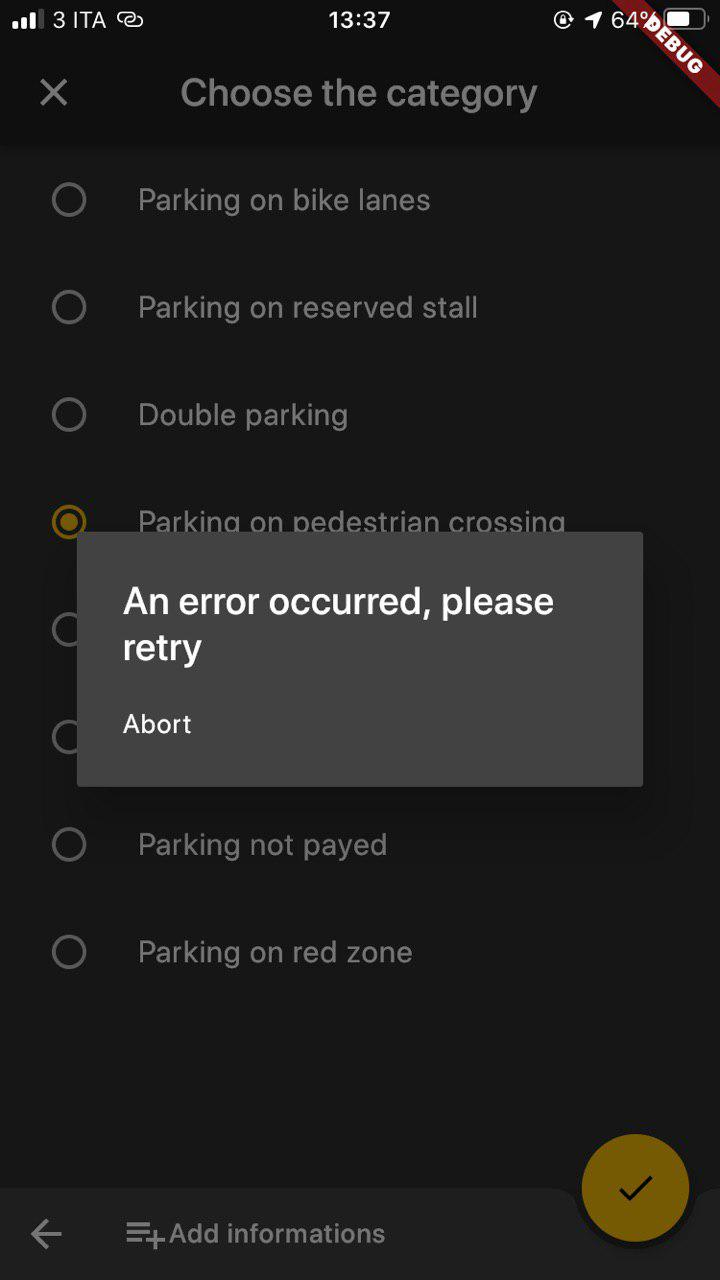
\includegraphics[scale = 0.3]{assets/report_upload_error.png}\\
        \caption[Report upload error]{Report upload error.}
    \end{figure}

    \subsection{Violation manipulation [R5]}\label{subsec:violation-manipulation.}
    R5: The system must avoid the manipulation of the violations.
    \newline
    Since it is impossible to upload a new violation, it is not possible to know if the system has manipulated the information.
    Anyway, a manipulation of data has been discovered indirectly in the application testing: when a municipality query the violation on its territory, sometimes some report are showed with the current date and time as upload date.
    We do not know what can cause this issue, since the violations seems to be stored correctly on the database.
    The test case that rose this issue is \textit{Municipality violation request 1}, from the previous section.
    In the follow is provided a screen of the error, as well as a the database actual situation.

    \begin{figure}[H]
        \centering
        \caption[Violation manipulation]{The first 5 violation show the date and time of the device (can be compared with the actual time on the top).}
    \end{figure}

    \begin{figure}[H]
        \centering
        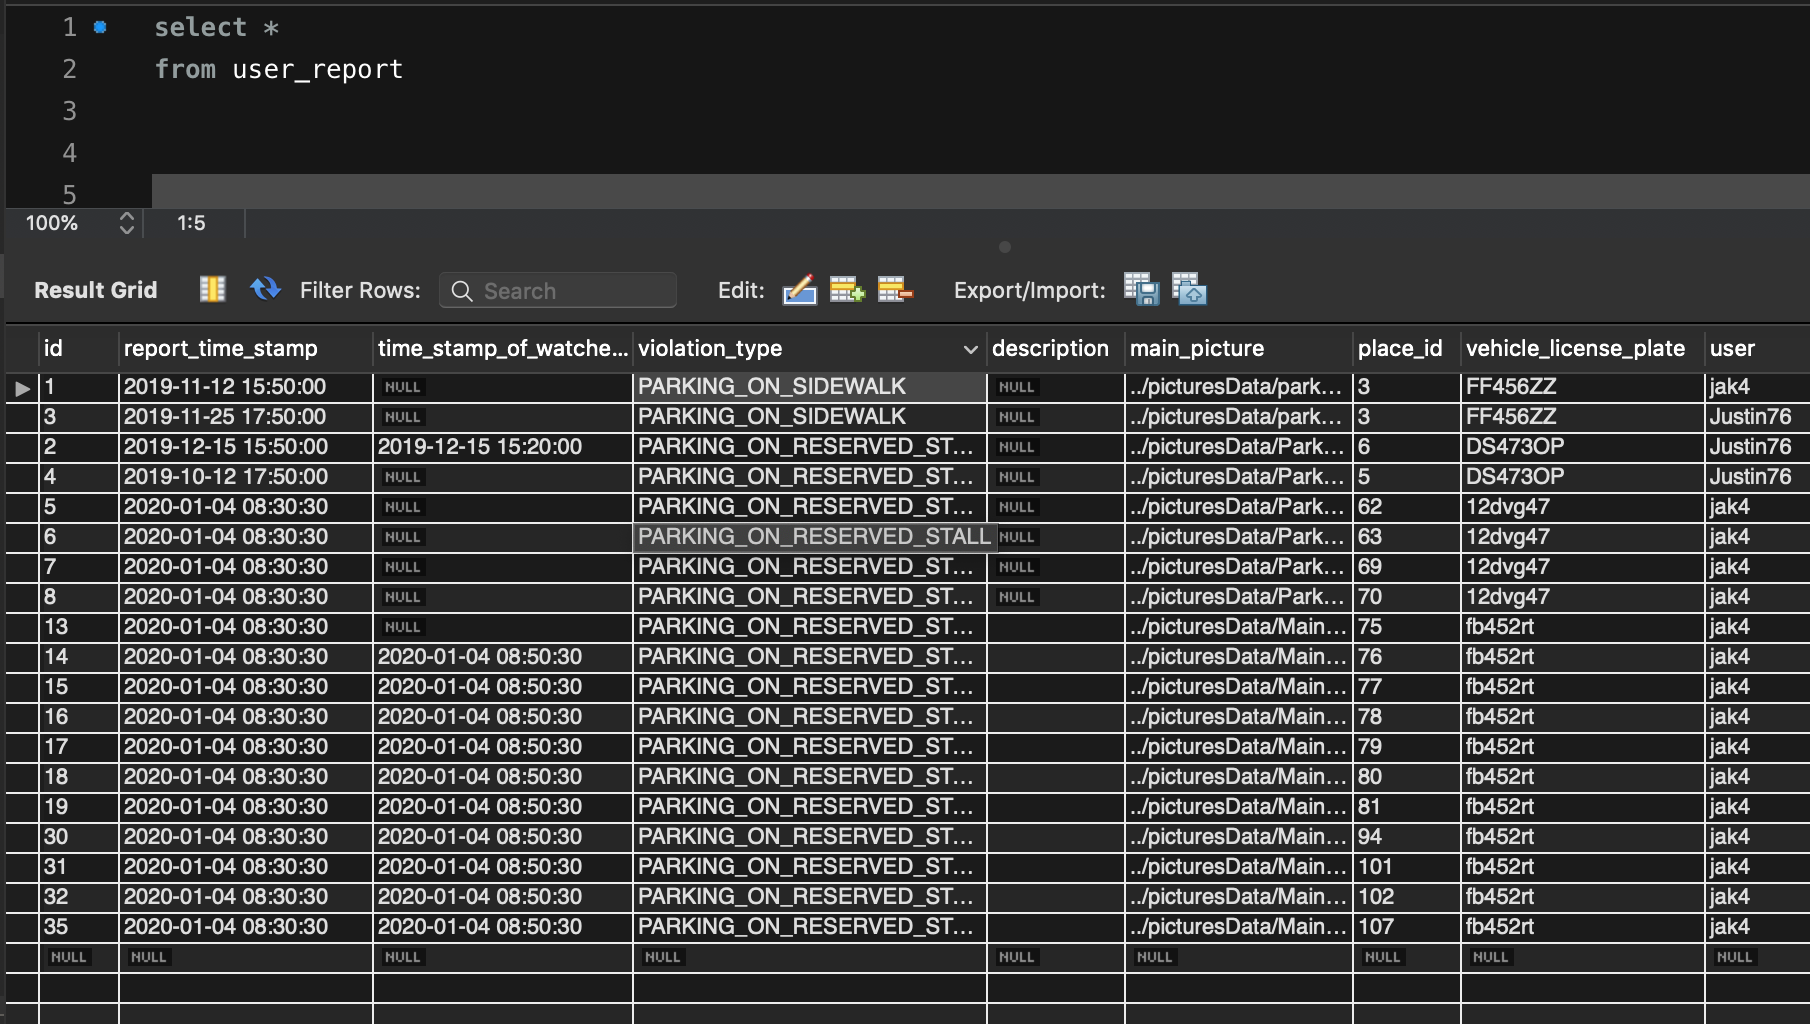
\includegraphics[scale = 0.5]{assets/database_user_report.png}\\
        \caption[Situation of the database]{Actual situation of the violation database while the test was running.}
    \end{figure}

    \subsection{Map and GPS [R6][R19]}\label{subsec:map-and-gps}
    R6: The system must be able to retrieve the position from the user or from the GPS.
    \newline
    R19: The System must communicate with the Maps Service.
    \newline
    This two requirements need to be presented together, since it is impossible to distinguish them for several issues of the application.
    \newline
    When the application run, after the user login, an error message is show in the "Arund me" main menu.
    The error shows up on every device we used to run the application: web page (Chrome, as indicated), android phone, iOS phone, iOS simulator.
    We think that this issue is related to the harvest of information about the user geolocation, and that it share the same cause with some other bug of the application (like the violation upload one), but this is just a firs analysis that can not be considered accurate without looking at the source code (that avoid the requirements of this document).
    In the following are showed some picture of the error.
    \newline
    \begin{figure}[H]
        \centering
        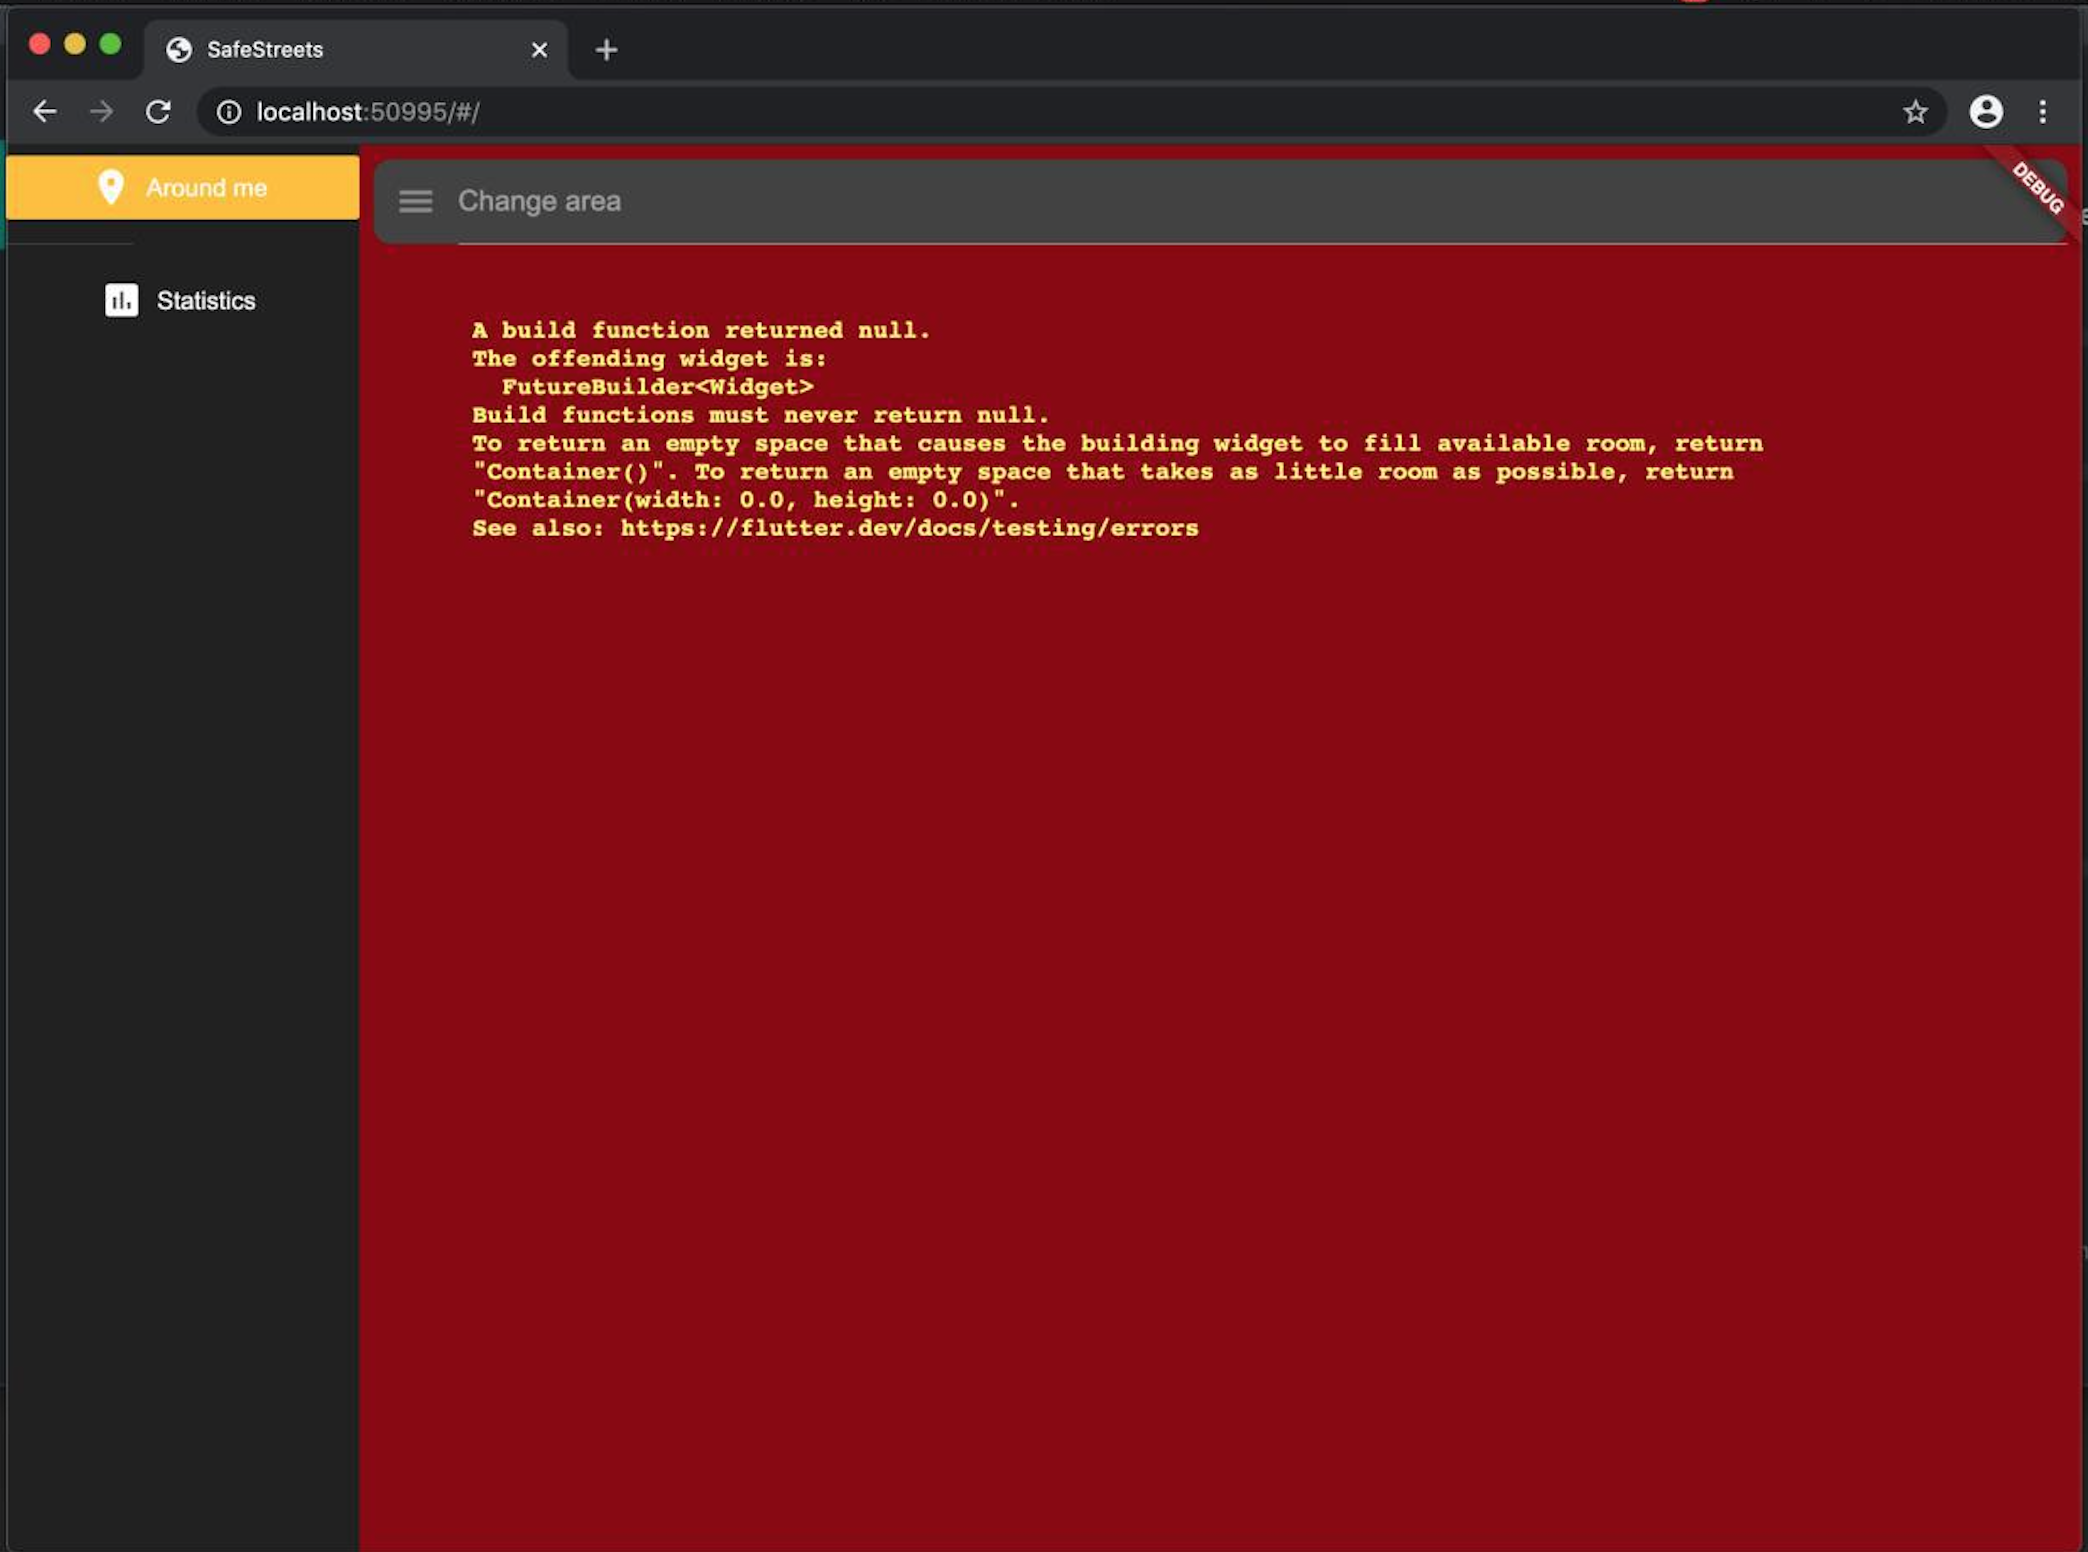
\includegraphics[scale = 0.4]{assets/web_page_error.png}\\
        \caption[Web page error]{Web page error.}
    \end{figure}

    \begin{figure}[H]
        \centering
        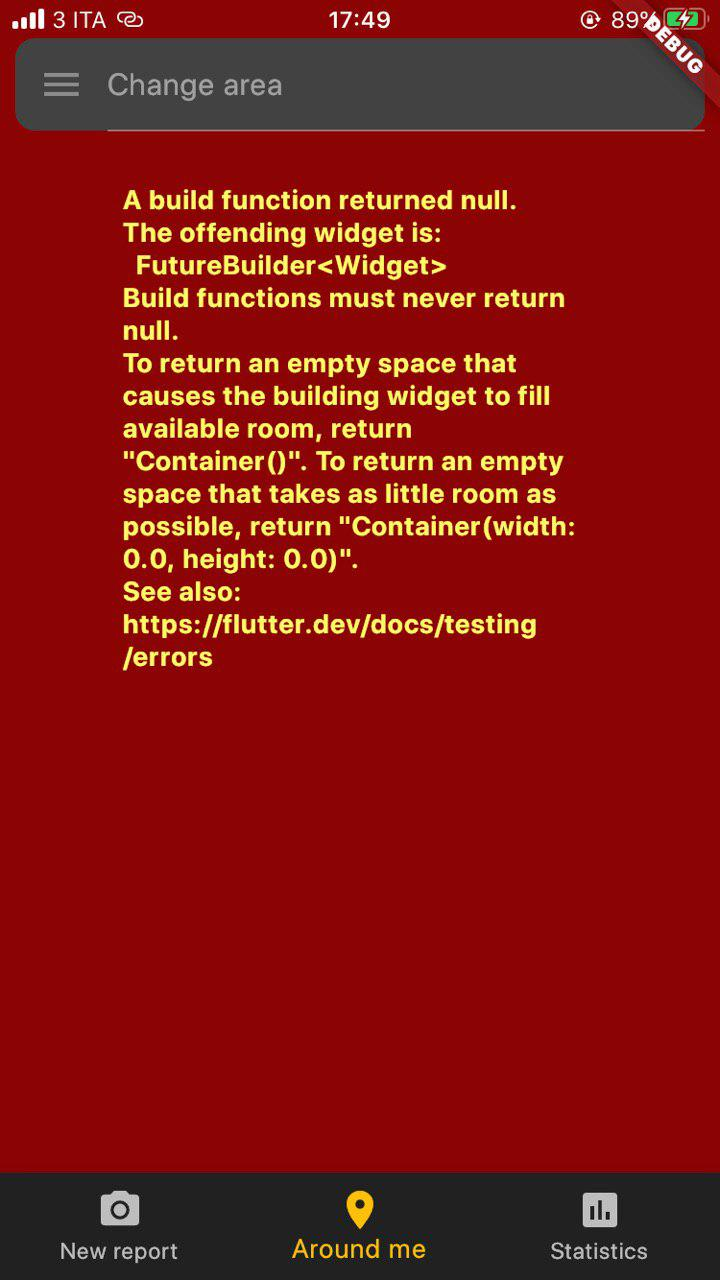
\includegraphics[scale = 0.25]{assets/smartphone_error.png}\\
        \caption[Smartphone error]{Smartphone error.}
    \end{figure}

    \begin{figure}[H]
        \centering
        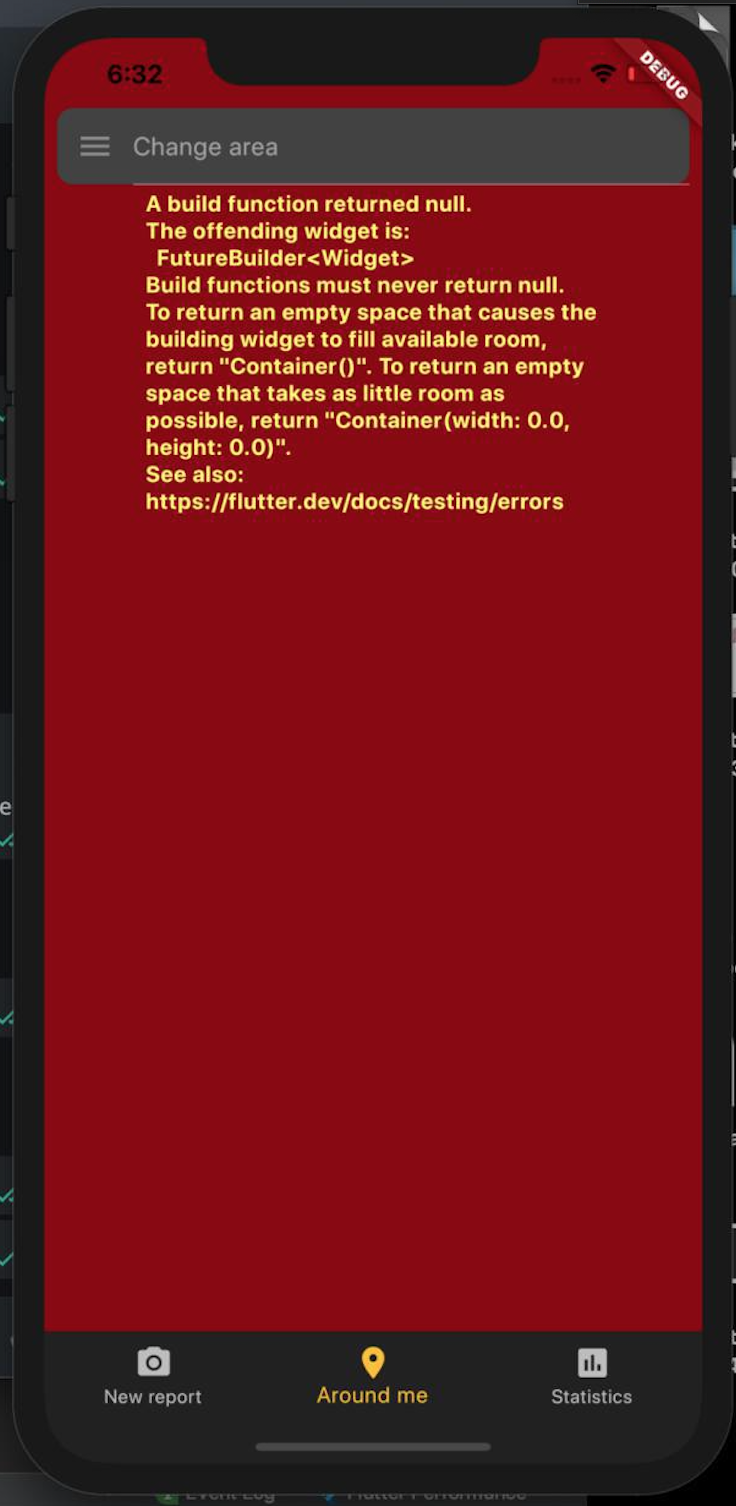
\includegraphics[scale = 0.4]{assets/iOS_simulator_error.png}\\
        \caption[iOS simulator error]{iOS simulator error.}
    \end{figure}

    The "Around me" menu should interface the user with the map, and it is not possible to say if this error comes from the GPS connection or the communication with the map service.
    By inserting a location in the text-bar on the top nothing happen, but it is reasonable to think that this is related to the bug already described.
    \newline
    The requirement R6 should concern even the violation upload by an user, that should be able to provide his location to associate it to the report.
    This is untestable, since it is not possible to reach that page in the upload phase.

    \subsection{Violation access [R7]}\label{subsec:violation-access}
    R7: Only the Municipality can access the submitted parking violation of its competence area
    \newline
    It is not possible to say if this requirement is satisfied.
    The only analysis that we can do is that the user can not see the "Access report" menu, but the main point of this requirement was probably on the possibility to see important information (like pictures or plate numbers) by the user, information that are not provided on these menu neither for the municipality.
    The issue of testing this requirement came from the error previously discussed of the "Around me" map, that we can not say what would show to the user, as well (less probably) as the statistics page.
    The requirement is so satisfied, but we can say nothing about what it would be without these two bugs.

    \subsection{Statistics calculation [R10]}\label{subsec:statistics-calculation}
    R10: The System must calculate some statistics:
    \newline
    R10.A: The system must calculate the streets with the highest and the lowest number of violations.
    \newline
    R10.B: The system must calculate the effectiveness of the service.
    \newline
    R10.C: The system must calculate the vehicles (identified by the traffic plate) that have committed the highest number of violations.
    \newline
    As showed in the previous section (\textit{Statistics [R2]}) the user can not see the statistics.
    This is enough to say that the requirement R2 (The user can view the statistics calculated by the System with some exceptions) is not satisfied, but not to say that the system is not able to build statistics, since it could just not show them.
    This consideration make the requirement impossible to be testes.
    \newline
    We did these consideration about this requirement because of its similarity with R2.
    In fact, considering a scenario in which the statistics are showed but they are incorrect, it would be satisfied only the requirement R2 and not the R10.

    \subsection{Violation acceptance}\label{subsec:violation-acceptance}
    R13: The system accepts only reports with a valid plate number and position.
    \newline
    This requirement should be only partially implemented (only accept a valid position).
    However, since it is not possible to upload a violation report, it is not possible to test it.

    \subsection{Non-mandatory attributes request}\label{subsec:non-mandatory-attribure-request}
    R16: The system must ask the User the non-mandatory attributes of the report.
    \newline
    The violation upload procedure can not be done, and it do not reach the page that should required the non mandatory attributes.
    Because of that, it is not possible to test this requirement.

\end{document}